% Define document class
\documentclass[manuscript]{aastex63}
\usepackage{tabularx}
\usepackage{amsmath}

\begin{document}

% Title
\title{Timing and Likelihood of the Origin of Life Derived from Post-Impact Highly Reducing Atmospheres}

% Authors
\author{Nicholas F. Wogan}
\affiliation{Department of Earth and Space Sciences, University of Washington, Seattle, WA 98195}
\affiliation{Virtual Planetary Laboratory, University of Washington, Seattle, WA98195}

\author{David C. Catling}
\affiliation{Department of Earth and Space Sciences, University of Washington, Seattle, WA 98195}
\affiliation{Virtual Planetary Laboratory, University of Washington, Seattle, WA98195}

\author{Kevin J. Zahnle}
\affiliation{Space Science Division, NASA Ames Research Center, Moffett Field, CA 94035}
\affiliation{Virtual Planetary Laboratory, University of Washington, Seattle, WA98195}

\begin{abstract}
Big impacts on the early Earth would have created highly reducing atmospheres that generated molecules needed for the origin of life, such as nitriles. However, such impactors can be followed by collisions that were still sufficiently big to vaporize the ocean and destroy any pre-existing life. Thus, a post-impact reducing atmosphere that gives rise to life needs to be followed by a lack of subsequent sterilizing impacts for life to persist. Using statistics and limits for the impact history on early Earth and the impact mass needed to generate post-impact highly reducing atmospheres, we show that the median timing of impact-driven biopoiesis (i.e., the origin of life) is favored early in the Hadean eon. However, uncertainties are large because impact bombardment is stochastic, so biopoiesis could have occurred in $\sim 0.5$ billion year window from 4.45 to 3.9 Ga within 95\% uncertainty. Previous claims of a far narrower window for the origin of life are unsupported. In an optimistic scenario for life starting from post-impact reducing atmospheres, we find that the origin of life is possible in $\sim 90\%$ of stochastic impact realizations. In our most pessimistic case, life's origin is still fairly likely ($\sim 20\%$ chance). This potentially bodes well for life on rocky planets elsewhere because they will have experienced an early episode of enhanced impact bombardment given how planets form.
\end{abstract}

\section{Introduction}

\citet{Benner_2020} argued that the most likely time for the origin of life in an RNA-world scenario would have been $4.36 \pm 0.1$ Ga in the wake of a $\sim 2 \times 10^{22}$ kg ($\sim 2100$ km) asteroid impact called Moneta. They suggested that iron delivered by Moneta's core would have reacted with impact-vaporized ocean water to generate a reducing Hadean atmosphere conducive to the photochemical generation of essential prebiotic nitriles like HCN and HCCCN. Nitriles are required in prebiotic schemes that synthesize ribonucleotide precursors to RNA \citep{Patel_2015,Powner_2009,Becker_2019}. A transient period of profuse nitrile production after a Moneta impact could have been a window of opportunity for the origin of RNA and, ultimately, life.

A single Moneta impact could also explain the highly-siderophile elements (i.e. iron-loving, abbreviated HSEs) in the Moon's and the Earth's mantles. During the Moon-forming impact, HSEs should have been sequestered in each planetary core, so over-abundant HSEs in today's mantles are commonly interpreted as evidence for late-accretion impactors. Earth's mantle has substantially more HSEs than the Moon by an amount that cannot be accounted for by Earth's greater gravitational cross section \citep{Day_2015}. A single massive Moneta impact could explain the Earth-Moon HSE discrepancy because, by the statistics of small numbers, Moneta could have missed the Moon and hit the Earth \citep{Sleep_1989,Bottke_2010}.

However, the lunar HSE depletion may be explained without a Moneta impact. Lunar HSEs could have been lost to space during impact-delivery because of the Moon's small gravity \citep{Kraus_2015}. Alternatively, HSEs delivered to the Moon during its $\sim 150$ million-year magma ocean could have been sequestered in the core due to iron sulfide exsolution \citep{Morbidelli_2018,Rubie_2016}. Finally, there is some chance that the Earth's HSEs do not record late impacts because the Moon-forming impact delivered HSEs \citep{Sleep_2016}. Another explanation for Earth's HSEs that does not require impacts is that HSEs are gradual core contributions over time from mantle plumes \citep{Halliday_2023,Mundl_2020}. If indeed Earth's HSEs reflect asteroid bombardment after the Moon formed, then the HSEs can be explained by multiple $\sim 500$ to 2000 km impacts rather than a single big ($\sim 2100$ km) collision.

Recently, \citet{Wogan_2023} and \citet{Zahnle_2020} used photochemical models of post-impact atmospheres to show that impacts significantly smaller than Moneta can efficiently produce prebiotic molecules. In their simulations, impactor iron equilibrates with vaporized ocean water to generate atmospheric H$_2$, CH$_4$ and NH$_3$ that form thermochemically as the reducing steam atmosphere cools. Once steam condenses to an ocean, subsequent photochemistry of a Titan-like, hazy atmosphere produces prebiotic nitriles. \citet{Zahnle_2020} was a preliminary study that used simple atmospheric models, and later \citet{Wogan_2023} improved upon their calculations with more sophisticated and accurate simulations. Photochemical modeling in \citet{Wogan_2023} shows that the production of both HCN and HCCCN only occurs when $\mathrm{CH_4} / \mathrm{CO_2} \gtrsim 0.1$ while the atmosphere is hazy. In an optimistic scenario, which includes nickel-catalyzed methane production, results suggests that $\mathrm{CH_4} / \mathrm{CO_2} > 0.1$ (i.e. significant nitriles) occurs for impacts $> 4 \times 10^{20}$ kg ($> 570$ km diameter). In a pessimistic case, which assumes only a fraction of impactor iron reacts with the atmosphere \citep{Citron_2022}, a $> 5 \times 10^{21}$ kg ($> 1330$ km diameter) impactor is required to produce substantial HCN and HCCCN \citep{Wogan_2023}. Regardless of uncertainty, atmospheric models suggest that an impactor much smaller than Moneta could deliver the nitriles needed for an RNA origin of life.

Here, we use the \citet{Wogan_2023} results, along with Monte-Carlo simulations of Earth's impact history, to make an alternative estimate for when life most likely emerged during an RNA-first process. Our calculations account for the possibility of planet sterilization by impacts that vaporize the ocean \citep{Sleep_1989}. We assume that a life-starting impact is one that produces significant prebiotic nitriles and is not subsequently followed by an ocean-vaporizing impact that destroys the biosphere. By considering the fraction of stochastic impact realizations that do not have a life-starting impact, we also estimate the probability of life beginning if Earth history was rerun.

\section{Methods} \label{sec:methods}
The rate impacts hit Earth bigger than mass $m$ at age $t$ can be written

\begin{equation}
  f(t,m) = F_0(t) S_0(m)
\end{equation}
Here, $S_0(m)$ is the size-frequency distribution of impactors normalized to a reference mass $m_0$ so that $S_0(m_0) = 1$. Also, $F_0(t)$ is the number of impacts per billion years with mass greater than $m_0$.

We assume that the the majority of the size-frequency distribution of impactors is identical to the main-belt asteroids \citep[Extended Data Figure 1 in][]{Marchi_2014}. Data for the frequency of main-belt asteroids only extends down to about 1 km diameter ($1.3 \times 10^{12} $ kg). To extend the distribution to smaller objects, we use the observed 1400 ratio between the frequency of $> 1$ km and $> 20$ km craters on the Moon following \citet{Morbidelli_2018}. Crater scaling relations suggest that 1 km and 20 km craters on the Moon corresponds to 50 m and 1 km asteroids, respectively \citep{Morbidelli_2018}. The largest main belt asteroid is $\sim 1000$ km, so we must extrapolate to larger impactors. Through the main text, we use the same extrapolation as \citet{Marchi_2014}, which extends the distribution to big impacts with a slope $d (\ln S_0)/d (\ln m) = - 0.415$ (Figure \ref{fig:sfd_and_flux}). In Appendix \ref{sec:append_sfd} we show that instead extrapolating with the red dashed line in Figure \ref{fig:sfd_and_flux}a (with slope $d (\ln S_0)/d (\ln m) = - 1.0$) does not significantly change our overall conclusions. Finally, we normalize the size-frequency distribution to the impact mass required to make a 1 km crater on the moon (50 m object, $m_0 = 1.64 \times 10^{8}$ kg). Figure \ref{fig:sfd_and_flux}a shows the resulting size-frequency distribution.

\begin{figure}
  \centering
  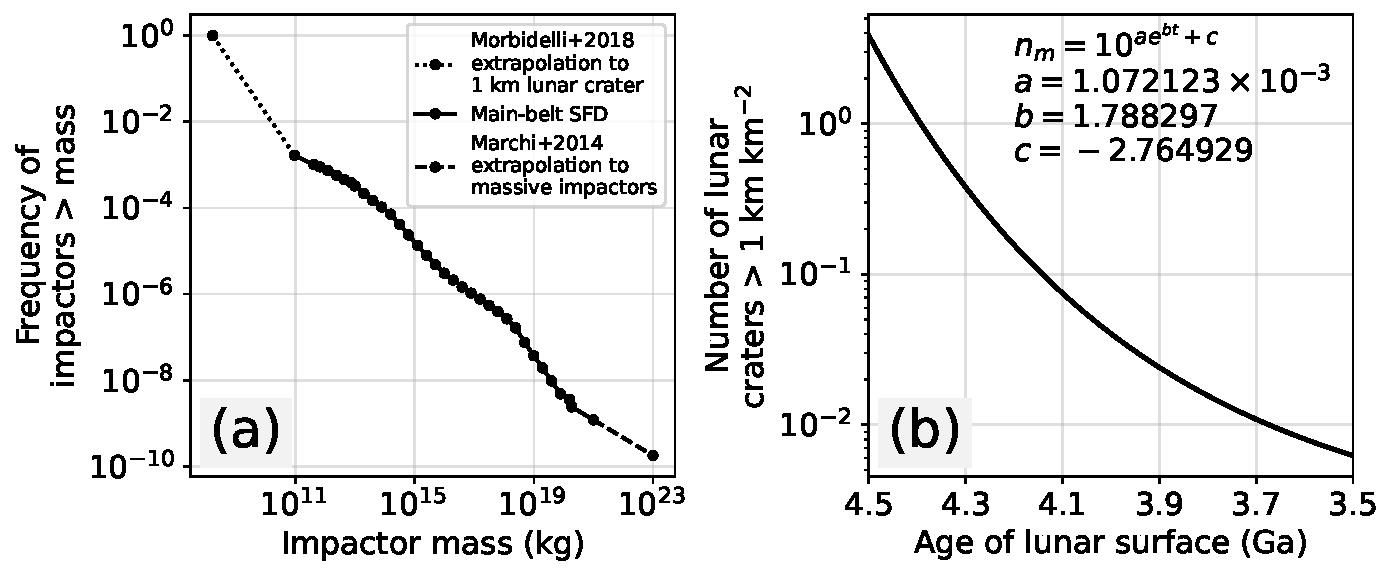
\includegraphics[width=1.0\textwidth]{figures/SFD_and_flux.pdf}
  \caption{Our assumed (a) size-frequency distribution of impactors and (b) lunar cratering record. Most of the size-frequency distribution is identical to the main-belt asteroids \citep[Extended Data Figure 1 in][]{Marchi_2014}. We extrapolate to objects $\lesssim 10^{11}$ kg using the observed frequency ratio of $> 1$ km and $> 20$ km lunar craters following \citet{Morbidelli_2018}, and, in the main text, log-log extrapolate to asteroids $\gtrsim 10^{21}$ kg following \citet{Marchi_2014}. In Appendix \ref{sec:append_sfd} we also consider the red dashed extrapolation to $\gtrsim 10^{21}$ kg impacts. The lunar cratering record is the red line in Figure 5 of \citet{Morbidelli_2018}.}
  \label{fig:sfd_and_flux}
\end{figure}

The flux of impactors, $F_0(t)$, can be estimated from the lunar cratering record. We adopt the accretionary tail scenario discussed in \citet{Morbidelli_2018}. In other words, we assume that the ``late heavy bombardment'' did not happen \citep{Cartwright_2022,Hartmann_2019,Zellner_2017}, and that the impact flux on Earth was monotonically decreasing throughout the Hadean eon. Figure \ref{fig:sfd_and_flux}b shows $n_m$, our assumed lunar impact history taken from \citet{Morbidelli_2018} (red line in their Figure 5). We use the parameterization $n_m = 10^{a e^{b t} + c}$, where $a$, $b$, and $c$ are fit parameters given in Figure \ref{fig:sfd_and_flux}b.

Extrapolating the lunar impact history to Earth requires correcting for Earth's greater gravitational attraction. Assuming that the approach velocity of impactors far from the Earth and Moon was on average 18 km/s \citep{Morbidelli_2018}, then Earth should receive $s_0 = 1.36$ times more impacts per surface area than the Moon. Therefore, the number of impacts on Earth is

\begin{equation}
  N_0 = A_\oplus s_0 n_m = A_\oplus s_0 10^{a e^{b t} + c}
  \label{eq:num_earth_impacts}
\end{equation}
Equation \eqref{eq:num_earth_impacts} also accounts for Earth's surface area ($A_\oplus$), making $N_0$ the number of impacts on Earth since age $t$ that would cause a crater $> 1$ km on the moon. As discussed previously, \citet{Morbidelli_2018} use crater scaling relations to show that a 1 km lunar crater corresponds to a 50 m object with mass $m_0 = 1.64 \times 10^8$ kg.

The time derivative of $N_0$ gives the flux, $F_0$:

\begin{equation}
  F_0(t) = \frac{d N_0}{dt}
\end{equation}
The average number of impacts on Earth between time $t_1$ and $t_2$ with mass greater than $m$ is then

\begin{align}
\begin{split}
  N(m,t_1,t_2) &= \int_{t_1}^{t_2} f(t,m) dt \\
  &= S_0(m) \int_{t_1}^{t_2} \frac{d N_0}{dt} dt \\
  &= S_0(m) A_\oplus s_0 \left( 10^{a e^{b t_2} + c} - 10^{a e^{b t_1} + c} \right)
\end{split}
\end{align}

To simulate impact histories, we consider a grid of $s\sim 200$ impactor masses between $10^{12}$ and $10^{23}$ kg, and a grid of $\sim 60$ times between 4.5 and 3.5 Ga. Indexes $j$ and $i$ indicate the mass and time grid cells respectively, while, for example, $j-\frac{1}{2}$ and $j+\frac{1}{2}$ indicate the edges of the grid cell. We can compute the expected number of impacts within a mass and time grid cell with the following

\begin{equation}
  \overline{N}_{ij} = N(m_{j-\frac{1}{2}},t_{i-\frac{1}{2}},t_{i+\frac{1}{2}}) - N(m_{j+\frac{1}{2}},t_{i-\frac{1}{2}},t_{i+\frac{1}{2}})
\end{equation}
Next, we sample a Poisson distribution for each $\overline{N}_{ij}$, giving a stochastic number of impacts in each mass and time grid cell which constitutes an impact history. By modeling impacts as a Poisson process, we are assuming that each impact does not change the probability of the next one (i.e., impacts are independent). Performing this sampling thousands of times captures many of the possible impact histories. We only keep impact histories that accrete a total mass of $2 \times 10^{22}$ to $6 \times 10^{22}$ kg because this is approximately the mass implied by the HSEs in Earth's mantle, assuming that HSEs were delivered by late accretion. This range of masses is based on \citet{Day_2015} who used mantle HSEs to suggest that the Earth was impacted by $\sim 3 \times 10^{22}$ to $4.8 \times 10^{22}$ kg of material, but we choose a wider range of masses because HSEs could have been lost to Earth's core or to space during impacts \citep{Marchi_2018}.

Our final step is to assign impact velocities to each collision in the many sampled impact histories. Appendix Figure \ref{fig:velocity_distribution} shows Earth's impact velocity distribution. We created this distribution using the JPL database of close approaches to Earth by small bodies \citep{Park_2023}, considering all close-approach asteroids within 0.05 AU to Earth. The database gives the approach velocity of each asteroid far from Earth, so we compute the impact velocity by accounting for Earth's gravitational potential energy. Here, we are assuming that the impact velocity distribution for small bodies (e.g. $< 10$ km) is identical to the velocity distribution for bigger asteroids (e.g. $> 10 km$). This may not be the case because small bodies are more strongly influenced by processes like the Yarkovsky effect \citep{Bottke_2006}, where an asteroid's orbit is altered by anisotropic thermal emission.

The final collection of sampled impact histories can then be used to compute impact statistics that are relevant to the timing and likelihood of the origin of life.

\section{Results} \label{sec:results}

\begin{figure}
  \centering
  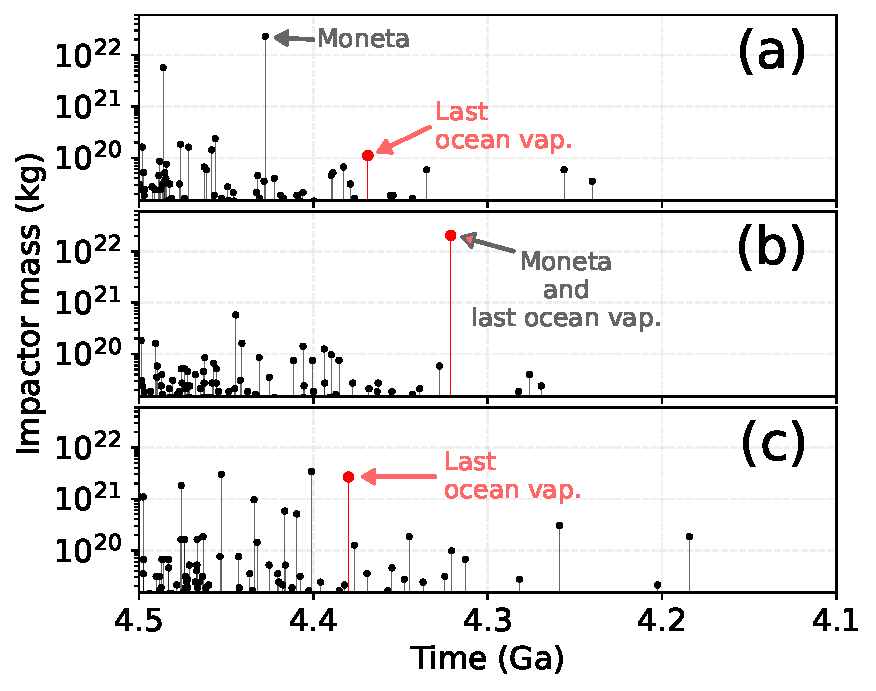
\includegraphics[width=0.65\textwidth]{figures/example_impact_histories.pdf}
  \caption{Three simulated impact histories of the 5000 derived from our Monte-Carlo approach (Section \ref{sec:methods}). Each vertical line indicates an impact of a mass shown by the y-axis. The red lines indicate the last impact to vaporize the ocean assuming 10\% of an impacts kinetic energy heats the ocean. (a) gives conversions between impact mass and diameter for 500, 1000 and 2000 km asteroids.}
  \label{fig:example_impact_histories}
\end{figure}

Figure \ref{fig:example_impact_histories} illustrates three of the 5000 impact histories computed with our Monte-Carlo approach (Section \ref{sec:methods}). In Figure \ref{fig:example_impact_histories}a, a Moneta-sized impact occurs at $\sim 4.43$ Ga delivering nearly all of Earth's mantle HSEs. The impact should also reduce the Hadean atmosphere creating conditions favorable for prebiotic chemistry. However, in this case, Moneta is not a life-starting impact because Moneta is followed by an ocean-vaporizing collision at $\sim 4.37$ Ga which we assume destroys any existing biosphere. Based on smoothed-particle hydrodynamics impact simulations, we nominally assume that 10\% of an impact's kinetic energy goes into vaporizing the ocean \citep[Appendix \ref{sec:append_vap},][]{Citron_2022}. Vaporizing the ocean requires $5 \times 10^{27}$ J, so a $> 5 \times 10^{28}$ J impact should deliver sufficient energy under our assumptions. Appendix \ref{sec:append_vap} considers alternative criteria for ocean-vaporization. In Figure \ref{fig:example_impact_histories}a, the last ocean-vaporizing impact is only $\sim 10^{20}$ kg (360 km) but has a large impact velocity of $32$ km/s giving it $5.12 \times 10^{28}$ J of kinetic energy. 

Moneta also occurs in the Figure \ref{fig:example_impact_histories}b impact realization. In this scenario, any life created in the wake of Moneta will not be subsequently impact-exterminated because Moneta is the last impact to vaporize the ocean.

Figure \ref{fig:example_impact_histories}c shows an impact history where Moneta does not occur. Instead, Earth's mantle HSEs are delivered by multiple $10^{21}$ to $4 \times 10^{21}$ kg collisions. Whether this bombardment history would cause biopoiesis depends on the required minimum impact mass to produce significant origin-of-life nitriles (e.g. HCN and HCCCN). \citet{Wogan_2023} uses photochemical models of post-impact atmospheres to show that, optimistically, an impact $> 4 \times 10^{20}$ kg should give rise to an atmosphere that makes significant HCN and HCCCN. Under this optimistic requirement, the last ocean-vaporizing impact in Figure \ref{fig:example_impact_histories}c could successfully start life and occurs at 4.38 Ga with mass $3 \times 10^{21}$ kg. However, with pessimistic modeling assumptions, \citet{Wogan_2023} finds that a $> 5 \times 10^{21}$ kg impactor is instead required for substantial nitrile delivery to the surface. In this alternative scenario, an origin of life never occurs in Figure \ref{fig:example_impact_histories}c because there is no impactor larger than $5 \times 10^{21}$ kg.

\begin{figure}
  \centering
  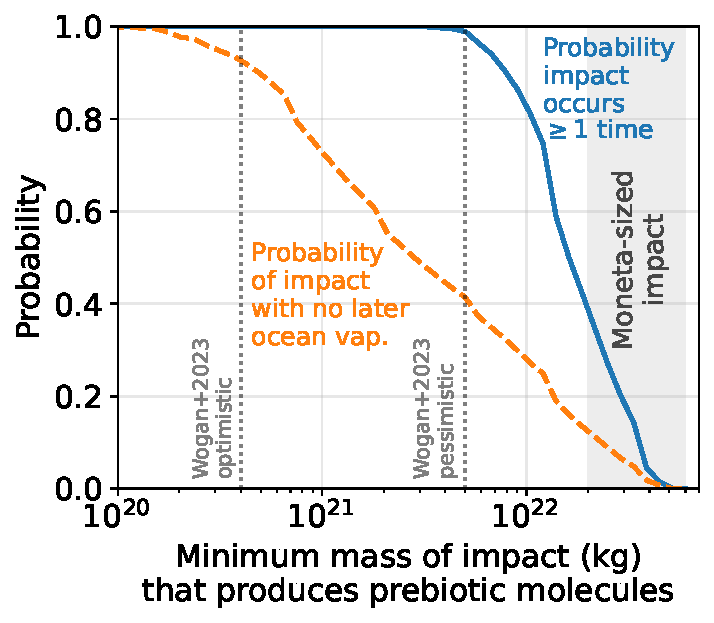
\includegraphics[width=0.5\textwidth]{figures/probabilities_of_impacts.pdf}
  \caption{The probability of an impact that causes favorable conditions for an origin of life on Earth. The blue solid line is the probability of an impact occurring at least once. The orange dashed line is the probability of an impact without a subsequent ocean-vaporizing collision. Probabilities are shown as a function of the minimum impact mass to produce significant prebiotic molecules (e.g. HCN). Two plausible minimum masses are the \citet{Wogan_2023} optimistic and pessimistic scenarios indicated with vertical dotted lines. The shaded region between $2 \times 10^{22}$ and $6 \times 10^{22}$ kg are Moneta-sized impacts because they deliver most all of Earth's mantle HSEs. There is a 92\% chance of an impact creating favorable origin of life conditions in the \citet{Wogan_2023} optimistic case, and a 41\% chance in the pessimistic case.}
  \label{fig:probabilities_of_impacts}
\end{figure}

As illustrated in Figure \ref{fig:example_impact_histories}, a life-starting impact does not occur in every simulated impact history. In our impact-driven model for the origin of life, biopoiesis requires (1) an impact of sufficient mass to make prebiotic nitriles and (2) the lack of a later ocean-vaporizing collision that destroys the biosphere without rekindling it. Figure \ref{fig:probabilities_of_impacts} shows the probability of both conditions occurring as a function of the minimum impact mass that produces prebiotic molecules. For example, consider the \citet{Wogan_2023} optimistic minimum mass of $4 \times 10^{20}$ kg indicated in Figure \ref{fig:probabilities_of_impacts}. All simulated impact histories have at least one impact bigger than $4 \times 10^{20}$ kg (blue line in Figure \ref{fig:probabilities_of_impacts} is 1.0 at the given mass). However, the probability of the origin of life in this scenario is 92\%, because 8\% of the time the last $4 \times 10^{20}$ kg collision is followed by a smaller ocean-vaporizing impact that perhaps sterilizes the planet (orange dashed line in Figure \ref{fig:probabilities_of_impacts} with 0.92 at $4 \times 10^{20}$ kg). An origin of life is less probable if we consider the \citet{Wogan_2023} pessimistic minimum mass ($> 5 \times 10^{21}$ kg) to produce significant origin-of-life nitriles. A $> 5 \times 10^{21}$ kg impact without later ocean vaporization occurs 41\% of the time. A life-starting impact was therefore relatively likely on the early Earth, and was strongly favored (92\% probability) under optimistic assumptions.

\begin{figure}
  \centering
  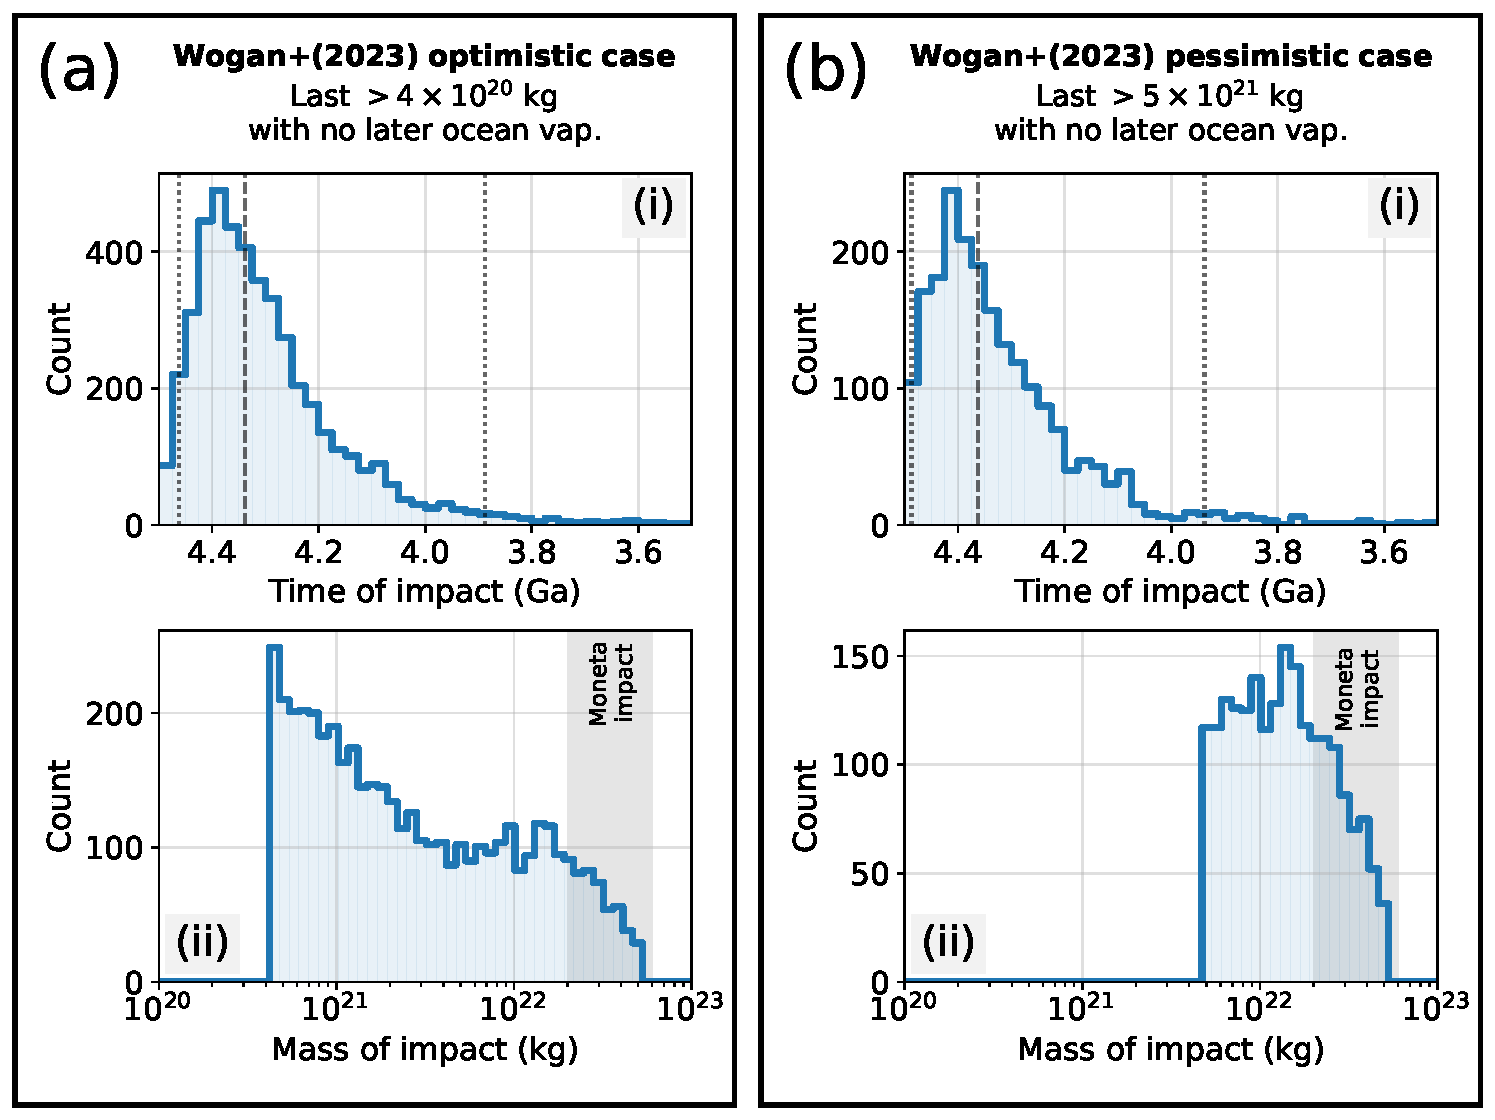
\includegraphics[width=0.85\textwidth]{figures/timing_and_mass.pdf}
  \caption{The timing and mass of a life-starting impact on the early Earth. (a) considers an optimistic minimum impact mass needed to generate the molecules for an RNA origin of life and (b) examines a pessimistic minimum impact mass \citep{Wogan_2023}. In either (a) or (b), panels (i) and (ii) show probability distributions for the timing and mass, respectively, of the last impact the produces prebiotic molecules which does not have a later ocean-vaporizing collision. The vertical dashed lines on (a) i and (b) i plot are median values, and the vertical dotted lines are the 95\% confidence intervals. In an impact-driven origin of life, biopoiesis most likely occurred at $4.34$ Ga (95\% CI: 3.89 to 4.46 Ga) assuming panel (a) and at $4.36$ Ga (95\% CI: 3.94 to 4.49 Ga) assuming panel (b).}
  \label{fig:time_and_mass}
\end{figure}

To estimate the most likely timing for the origin of life, we consider both the optimistic and pessimistic criteria of \citet{Wogan_2023}. Figure \ref{fig:time_and_mass}a is the optimistic case, showing the timing (Figure \ref{fig:time_and_mass}a (i)) and mass (Figure \ref{fig:time_and_mass}a (ii)) of the last $> 4 \times 10^{20}$ kg impactor for the 92\% of impact histories that do not experience later ocean vaporization. The median timing of a life-starting impact is 4.34 Ga with 95\% uncertainty between 3.89 and 4.46 Ga. The large uncertainty mostly stems from the stochastic, Poisson nature of asteroid bombardment. The probability distribution for the mass of the life-starting impact peaks at $4 \times 10^{20}$ kg and decreases with increasing mass because of the size-frequency distribution of asteroids (Figure \ref{fig:sfd_and_flux}a). There is only a 10\% chance that the impactor is Moneta-sized (i.e., between $2 \times 10^{22}$ and $6 \times 10^{22}$ kg).

The timing of an origin of life impact is qualitatively unchanged when instead adopting the \citet{Wogan_2023} pessimistic case, which requires a $> 5 \times 10^{21}$ kg impact without later ocean vaporization (Figure \ref{fig:time_and_mass}b). In this scenario, the median timing for life's origin is 4.36 Ga with a 95\% confidence interval spanning 3.94 to 4.49 Ga (Figure \ref{fig:time_and_mass}b (i)). Under these assumptions, the life-starting impact is Moneta-sized 31\% of the time (Figure \ref{fig:time_and_mass}b (ii)), which is more probable compared to ``optimistic'' case (Figure \ref{fig:time_and_mass}a (ii)).

In this model for biopoiesis, life would probably start approximately within 10s of millions of years after a life-starting impact because this is the maximum duration of the H$_2$- and CH$_4$- rich atmosphere that makes nitriles like HCN \citep{Wogan_2023}. We ignore the $< 10$s million year span between an impact and life's origin because it is small compared to our $\sim 500$ million-year uncertainty for the timing of a life-starting impact.

\section{Discussion}

Our estimated timing for biopoiesis is compatible with the earliest well-accepted geologic evidence of life in the form of stromatolites in the 3.5 Ga Pilbara block of western Australia \citep{Walter_1980,Buick_1981,Van_2018}. Older geologic evidence of life exists, such as a $> 3.7$ Ga black shale metamorphosed to graphite with negative $\delta^{13}$C characteristic of biology \citep{Rosing_1999,Ohtomo_2014}. Also, \citet{Bell_2015} discovered graphite inclusions in a 4.1 Ga zircon grain with $^{13}$C depletions compatible with biological activity, but this is a tentative biosignature because there are abiotic mechanisms for making isotopically light carbon \citep{Javaux_2019}. If the \citet{Bell_2015} finding is indeed a sign of life, then it would be generally compatible with our estimated timing in Figure \ref{fig:time_and_mass}, because we find that there is only a $\sim 10\%$ chance of life starting after 4.1 Ga.

Furthermore, Hadean zircons provide some constraint on Earth's impact history which we do not explicitly account for in our calculations. The oldest zircons are from Jack Hills, Australia, with U-Pb dates as old as $\sim 4.38$ Ga \citep{Valley_2014}. \citet{Benner_2020} argued that a Moneta-scale impact ($\sim 2 \times 10^{22}$ kg) could not have occurred after this date, because such a collision would heat the crust enough to potentially reset all U-Pb chronometers. \citet{Benner_2020} makes this claim based on \citet{Abramov_2013}, who used models of impact ejecta coupled to simulations of radiogenic Pb-loss in zircons to investigate chronometers resetting during the hypothesized ``late-heavy bombardment''. However, \citet{Abramov_2013} considers impacts much smaller than Moneta (e.g. $< 10^{21}$ kg), and does not clearly establish a minimum impactor mass that would reset all zircon chronometers globally. Given this ambiguity, our simulations do not use zircon chronometers as a constraint on Earth's impact history.

Even if an impact failed to reset a zircon chronometer, the shock wave produced by an asteroid collision may create micro- to nano-structural features in zircons that could be preserved over billions of years \citep{Reimink_2023}. Therefore, the presence or absence of shocked Hadean zircons in the geologic record may provide some constraint on Earth's impact history. For example, \citet{Reimink_2023} estimated the probability of preserved zircons with shock features assuming Earth experienced a ``late-heavy bombardment'' at 3.9 Ga. In this scenario, they find that shocked zircons were likely preserved yet find none in a collection of 4.02 Ga zircons from the Acasta Gneiss Complex. Overall, the absence of preserved shocked zircons suggests that a ``late-heavy bombardment'' did not occur at 3.9 Ga. Our Monte-Carlo models of Earth's impact history do not use zircon shock features as a constraint. A better model would incorporate this information.

It is temping to extrapolate our results beyond the early Earth to exoplanets, but we must do so with caution because planets orbiting different stars may have bombardment histories unlike the Hadean. Planets in the habitable zone of a late M-type star during the stellar main-sequence phase were interior to the habitable zone for several hundred million years during the super luminous pre-main-sequence phase \citep{Luger_2015}. \citet{Lichtenberg_2022} use N-body simulations to show that, for planets hosted by late M-dwarfs, large asteroid impacts are not useful for prebiotic chemistry because big impacts most likely occur within 100 million years of planet formation during the stellar pre-main-sequence when the planet is outside of the habitable zone. The pre-main-sequence phase is not an issue for an impact-induced origin of life on planets orbiting sun-like stars because the phase only lasts $\sim 3$ Myrs, while large asteroid impacts occur for 100s Myrs \citep{Lichtenberg_2022}. Therefore, our result that a life-starting impact was likely on the early Earth (92\% chance in an optimistic case) might be best extrapolated to habitable zone exoplanets orbiting sun-like stars.

A caveat to our results is that ocean-vaporization by an impact is likely a complicated function of impact mass, velocity, and incident angle, which we do not account for (Appendix \ref{sec:append_vap}). Throughout Section \ref{sec:results} we have assumed that 10\% of an impactor's kinetic energy heats the planetary surface ($f_\mathrm{E,vap} = 0.1$), leading to a required $> 5 \times 10^{28}$ J collision to vaporize an ocean. Appendix Figure \ref{fig:energy_for_ocean_vap} uses simulations of impacts from \citet{Citron_2022} to show that $f_\mathrm{E,vap} = 0.1$ is a reasonable assumption, but that values between 2.5\% and 25\% are also possible and that $f_\mathrm{E,vap}$ likely also depends on impact angle.

To determine the sensitivity of our results to $f_\mathrm{E,vap}$, we recomputed the likelihood and timing of an impact that starts life in Appendix \ref{sec:append_vap} using $f_\mathrm{E,vap} = 0.025$ and $f_\mathrm{E,vap} = 0.25$. We find that the probability of a life-starting impact is somewhat sensitive to $f_\mathrm{E,vap}$, while the timing does not depend strongly on $f_\mathrm{E,vap}$. Overall, this uncertainty does not change our qualitative conclusion that an origin of life impact on the early Earth was not a fluke. Even in our worst-case scenario (i.e., \citet{Wogan_2023} pessimistic case with $f_\mathrm{E,vap} = 0.25$) a life-starting impact occurs in 20\% of impact realizations (Appendix Figure \ref{fig:probabilities_of_impacts_sens}). Additionally, uncertainty in $f_\mathrm{E,vap}$ does not change our general conclusion that the most likely timing for the origin of life was $\sim 4.35$ Ga, with 95\% uncertainty spanning the Hadean eon (Appendix Figure \ref{fig:timing_sensitivity}). However, a more complete understanding of $f_\mathrm{E,vap}$ as a function of impact angle and other similar parameters may change this result.

An additional related caveat is that our calculations assume that an impact that vaporizes the ocean also sterilizes the planet, but this may not be the case because microbes might have survived in the deep subsurface \citep{Sleep_1989,Grimm_2018}. If ocean-vaporization does not destroy the biosphere, then our results would favor an origin of life earlier than we predict in Figure \ref{fig:time_and_mass}, and a life-starting impact would also be more probable than we have estimated (Figure \ref{fig:probabilities_of_impacts}).

\section{Conclusions}

We use Monte-Carlo simulations of Earth's impact history to determine the most likely timing for the origin of life that requires early ribonucleobase synthesis. We use the results of \citet{Wogan_2023}, who find that significant origin of life precursor molecules, such as HCN, are produced in the Hadean atmosphere after a $> 4 \times 10^{20}$ kg impact in an optimistic case, and after a $> 5 \times 10^{21}$ kg impact in a pessimistic scenario. We consider both possibilities, and assume such impacts can cause life's origin so long as they are not followed by a smaller ocean-vaporizing collision that sterilizes the planet.

For either the optimistic or pessimistic cases, we find that the most likely timing for an origin of life impactor is $\sim 4.35$ Ga with a 95\% uncertainty spanning the entire Hadean eon (approximately 4.45 to 3.9 Ga). The large uncertainty is caused by the intrinsic stochastic nature of impacts. These results suggest that the \citet{Benner_2020} proposed timing of the origin of life, at $4.36 \pm 0.1$ Ga, is too narrow. Furthermore, the mass of the life-starting impactor is most likely (69\% to 90\% probability) smaller than the Moneta impactor (Figure \ref{fig:time_and_mass}) proposed by \citet{Benner_2020}, because the size frequency distribution of asteroids prefers more frequent smaller impactors.

Our simulations of Earth's impact history do not always result in a bombardment favorable for an origin of life. There are some impact histories where a collision of sufficient mass to produce prebiotic molecules does not occur, or alternatively, does occur but primitive life is subsequently destroyed by an ocean-vaporizing impact that does not rekindle the biosphere. With our nominal assumptions, a life-starting impact occurs 92\% or 41\% of the time when we assume a $> 4 \times 10^{20}$ kg or $> 5 \times 10^{21}$ kg impact without later ocean-vaporization is required to start life, respectively. In our worst-case scenario, which assumes that impacts can more easily vaporize the ocean, a $> 5 \times 10^{21}$ kg impact without subsequent planet sterilization occurs in 20\% of simulated impact histories (Appendix Figure \ref{fig:probabilities_of_impacts_sens}).

If life began after an impact that generated a reducing atmosphere, then this work suggests that origin of life on Earth was fairly likely (at least a 20\% chance) and was indeed strongly favored (92\% chance) under optimistic assumptions. Given that rocky planets form from accretionary impacts, our work supports an optimistic outlook for life on exoplanets orbiting sun-like stars and future searches for biosignatures. 

\section*{Acknowledgements}

We thank Roger Buick for reading an early draft of this article and providing useful feedback. N.F.W. and D.C.C. were supported by the Simon's Collaboration on Origin of Life Grant 511570 (to D.C.C.). Also, N.F.W., D.C.C., and K.J.Z. were supported by NASA Astrobiology Program Grant 80NSSC18K0829 and benefited from participation in the NASA Nexus for Exoplanet Systems Science research coordination network. N.F.W. and D.C.C. also acknowledge support from Sloan Foundation Grant G-2021-14194.

\appendix

\renewcommand{\thefigure}{A\arabic{figure}}
\renewcommand{\thetable}{A\arabic{table}}
\setcounter{figure}{0}
\setcounter{table}{0}

\begin{figure}
  \centering
  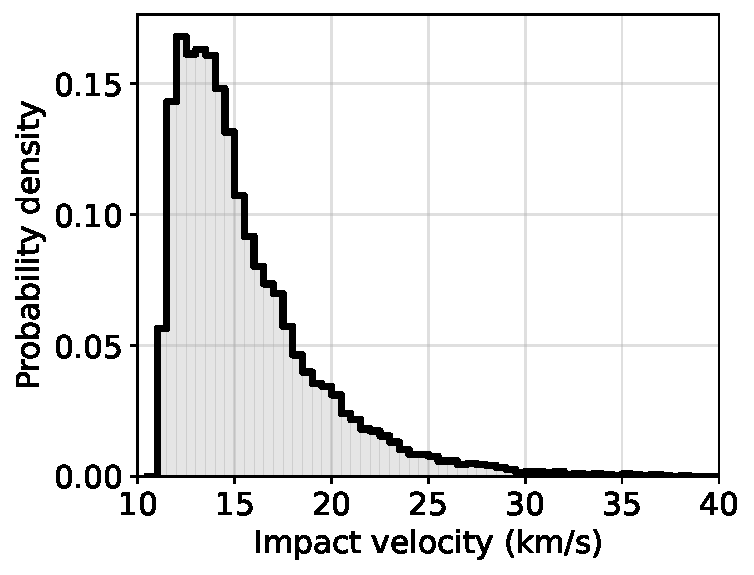
\includegraphics[width=0.4\textwidth]{figures/velocity_distribution.pdf}
  \caption{Our assumed probability distribution for the velocity of impacts derived from modern observations of asteroid close approaches \citep{Park_2023}.}
  \label{fig:velocity_distribution}
\end{figure}

\section{Size-frequency distribution sensitivity test} \label{sec:append_sfd}

We assume that the size-frequency distribution of objects that struck the early Earth is similar to the main-belt asteroids. A problem with this approach is that the main-belt asteroids only contain objects up to $\sim$ 1000 km diameter, yet the early Earth is expected to have experience impacts larger than this \citep{Marchi_2014}. Therefore, we must extrapolate the size-frequency distribution above $\sim$ 1000 km to larger objects. Throughout the main text we use the same extrapolation as \citet{Marchi_2014} (the black dashed line in Figure \ref{fig:sfd_and_flux}), who extends the size-frequency distribution with a log-log slope of $d (\ln S_0)/d (\ln m) = - 0.415$.

To test the sensitivity of our results to this chosen extrapolation, we re-did our Monte-Carlo analysis using a log-log slope of $d (\ln S_0)/d (\ln m) = - 1$ (the red dashed line in Figure \ref{fig:sfd_and_flux}) for impactors bigger than $\sim$ 1000 km diameter. Figures \ref{fig:probabilities_of_impacts_extrapolation_sens} and \ref{fig:timing_extrapolation_sensitivity} show how our results change when adopting this alternative extrapolation. Overall, our results are qualitatively unchanged for the different extrapolation slope ($d (\ln S_0)/d (\ln m)$).

\begin{figure}
  \centering
  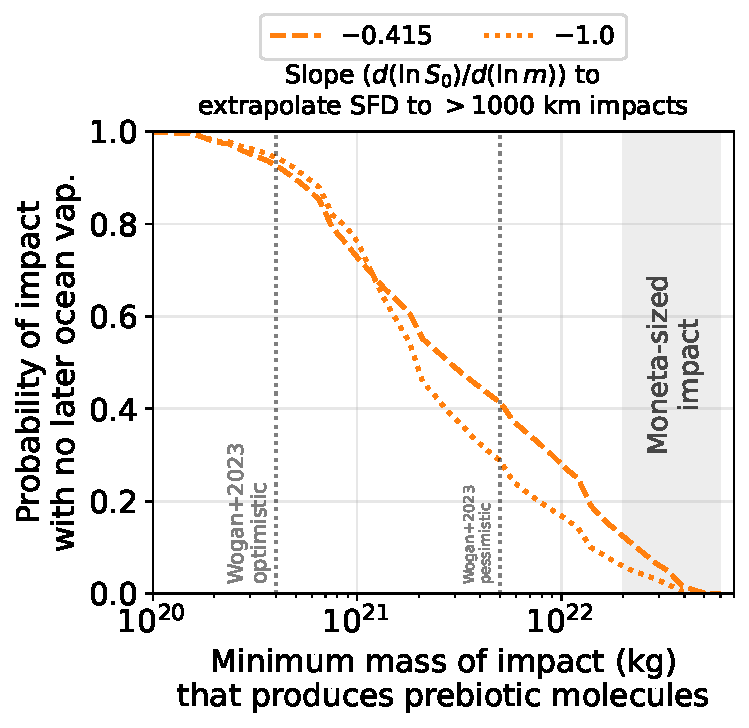
\includegraphics[width=0.5\textwidth]{figures/probabilities_of_impacts_extrapolation_sens.pdf}
  \caption{Similar to Figure \ref{fig:probabilities_of_impacts}, except we consider different extrapolations of the size-frequency distribution (SFD) for impactors larger than 1000 km diameter. The line labeled $d (\ln S_0)/d (\ln m) = - 0.415$ is the black dashed extrapolation in Figure \ref{fig:sfd_and_flux}a. The $d (\ln S_0)/d (\ln m) = - 1.0$ case is shown by the red dashed extrapolation in Figure \ref{fig:sfd_and_flux}a.}
  \label{fig:probabilities_of_impacts_extrapolation_sens}
\end{figure}

\begin{figure}
  \centering
  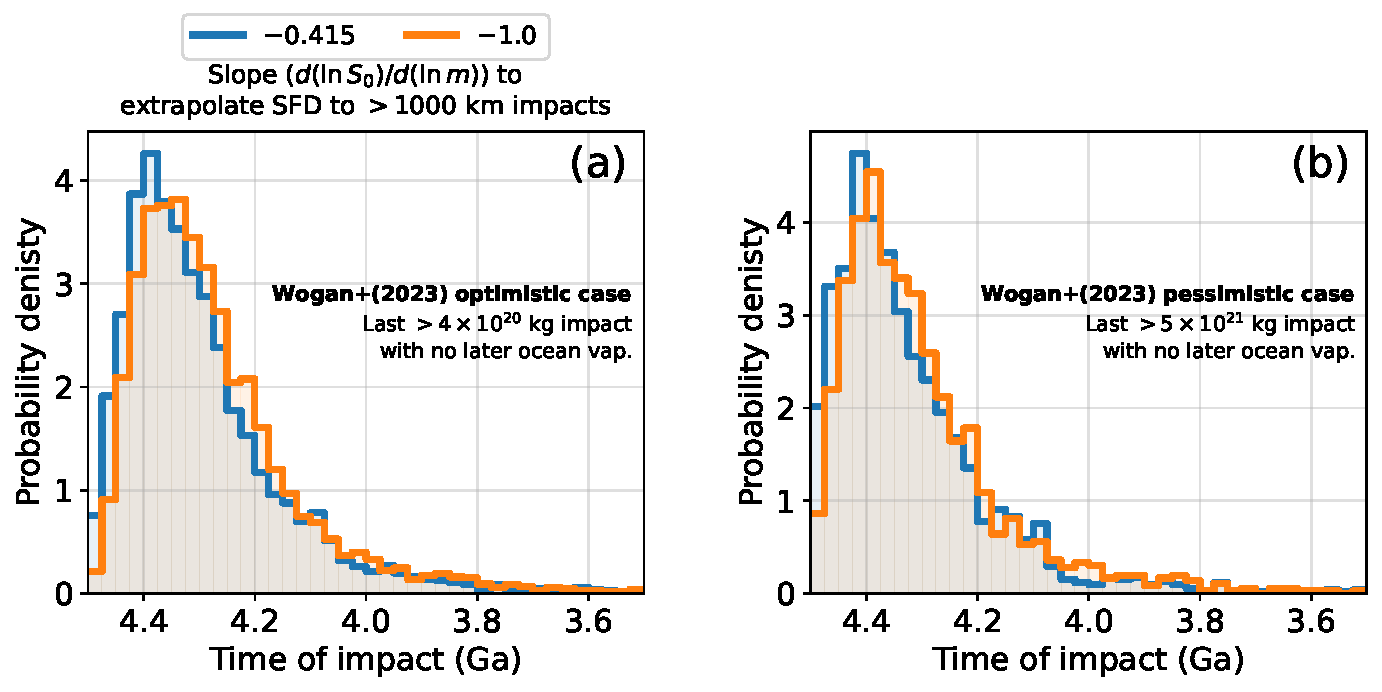
\includegraphics[width=0.85\textwidth]{figures/timing_extrapolation_sensitivity.pdf}
  \caption{Similar to Figure \ref{fig:time_and_mass}, except we consider different extrapolations of the size-frequency distribution (SFD) for impactors larger than 1000 km diameter. The line labeled $d (\ln S_0)/d (\ln m) = - 0.415$ is the black dashed extrapolation in Figure \ref{fig:sfd_and_flux}a. The $d (\ln S_0)/d (\ln m) = - 1.0$ case is shown by the red dashed extrapolation in Figure \ref{fig:sfd_and_flux}a.}
  \label{fig:timing_extrapolation_sensitivity}
\end{figure}

\section{Impact energy required for ocean vaporization} \label{sec:append_vap}

Recently, \citet{Citron_2022} performed smoothed-particle hydrodynamics impact simulations over a range of impact angles, masses and velocities to estimate the impact properties that can vaporize an ocean. Figure \ref{fig:energy_for_ocean_vap}a shows their simulation results for the change in the atmosphere's and ocean's internal energy ($\Delta \mathrm{IE}_\mathrm{atmo}$) as a function of impact kinetic energy ($\mathrm{E}_\mathrm{imp}$), along with log-log extrapolations for each impact angle. Figure \ref{fig:energy_for_ocean_vap} gives the same information, but the y-axis is instead the fraction of the impactor's energy that heats the atmosphere and ocean over the course of their simulations. For the most probable incident impact angle of $45^\circ$ about $\sim 10\%$ of the impactors kinetic energy heats the atmosphere ($f_\mathrm{E,vap} = 0.1$), so we nominally adopt this value in the main text to determine which collisions vaporize the ocean.

Energy delivery to the atmosphere/ocean appears to depend on impact angle, mass and velocity (Figure \ref{fig:energy_for_ocean_vap}). Additionally, all of the \citet{Citron_2022} simulations are far more massive than the minimum threshold for ocean-vaporization, so we must rely on extrapolations. Therefore, our assumption of a constant $f_\mathrm{E,vap} = 0.1$ is an over-simplification. To remedy this shortcoming, we considered building a parameterization for $f_\mathrm{E,vap}$ that depends on multiple impact properties (e.g., impact angle) using the \citet{Citron_2022} simulation results, but this was unsuccessful because their calculations do not consider a wide enough parameter space.

\begin{figure}
  \centering
  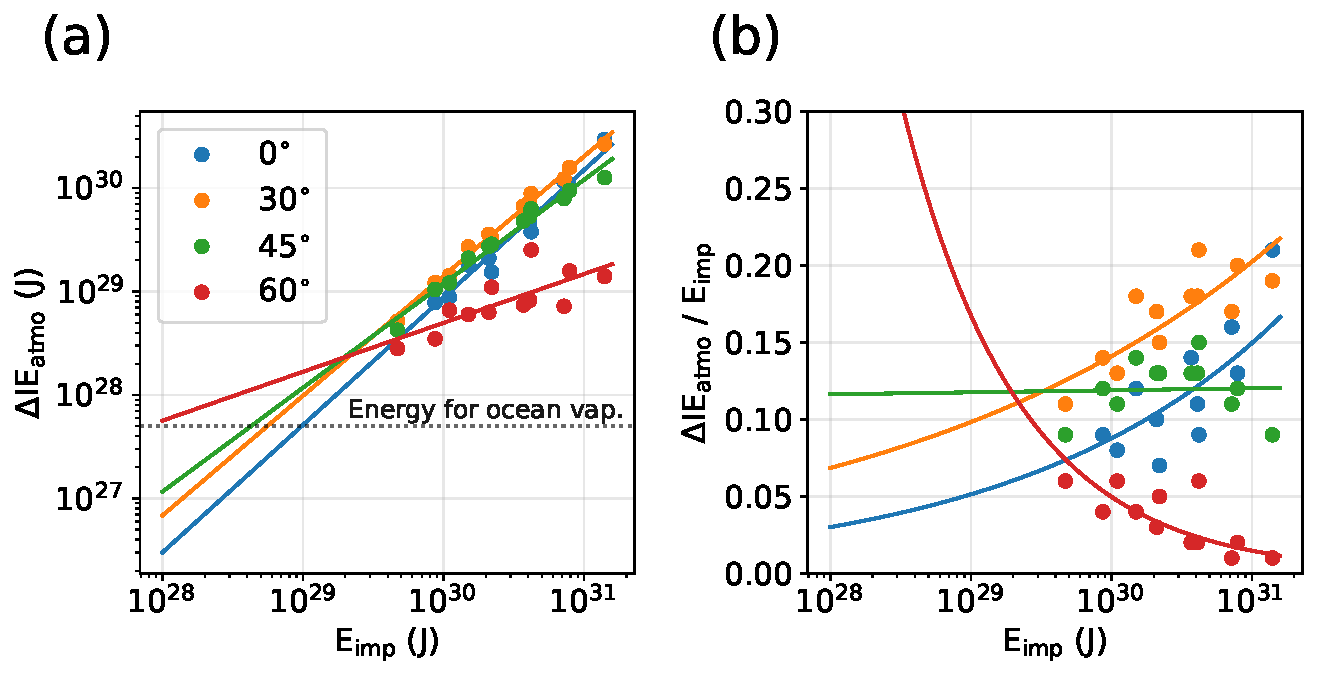
\includegraphics[width=0.8\textwidth]{figures/energy_for_ocean_vap.pdf}
  \caption{\citet{Citron_2022} smoothed-particle hydrodynamics simulations that show how much impactor kinetic energy heats the atmosphere and ocean. Different colors indicated various incident impact angles. (a) shows the simulated change in internal energy of the atmosphere and ocean as a function of the impactor energy, with linear log-log extrapolations for each impact angle. The dotted horizontal line at $5 \times 10^{27}$ J indicates the energy needed to vaporize an ocean \citep{Sleep_1989}. (b) contains the same information as (a), except the y-axis is the fraction of impactor energy that heats the atmosphere and ocean.}
  \label{fig:energy_for_ocean_vap}
\end{figure}

The evaluate the sensitivity of our results to an assumed constant $f_\mathrm{E,vap} = 0.1$, we recomputed the likelihood and timing of a life-starting impact using $f_\mathrm{E,vap} = 0.025$ and $f_\mathrm{E,vap} = 0.25$ (Figure \ref{fig:probabilities_of_impacts_sens} and \ref{fig:timing_sensitivity}). We chose these values because they are reasonable lower and upper bounds based on the \citet{Citron_2022} simulations (Figure \ref{fig:energy_for_ocean_vap}b). The probability of an impact that produces substantial prebiotic molecules without later ocean vaporization decreases with increasing $f_\mathrm{E,vap}$ (Figure \ref{fig:probabilities_of_impacts_sens}). For example, for $f_\mathrm{E,vap} = 0.1$, the probability of a $>4 \times 10^{20}$ kg impact (\citet{Wogan_2023} optimistic case) without subsequent ocean vaporization is 92\%. For $f_\mathrm{E,vap} = 0.025$ and $f_\mathrm{E,vap} = 0.25$ the probabilities are instead 99.9\% and 60\%, respectively.

\begin{figure}
  \centering
  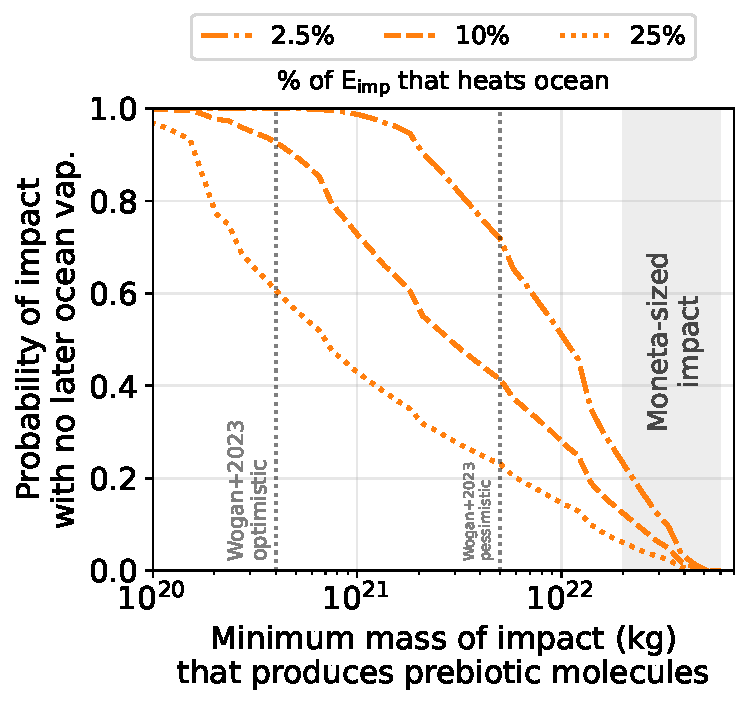
\includegraphics[width=0.5\textwidth]{figures/probabilities_of_impacts_sens.pdf}
  \caption{Similar to Figure \ref{fig:probabilities_of_impacts}, except we consider different values for the fraction of impactor energy that heats the ocean.}
  \label{fig:probabilities_of_impacts_sens}
\end{figure}

Figure \ref{fig:timing_sensitivity} shows the timing of the last impact to make conditions favorable for biopoiesis that does not experience subsequent ocean vaporization for $f_\mathrm{E,vap}$ values of 0.025, 0.1 (nominal value), and 0.25. As in the main text, we consider the \citet{Wogan_2023} optimistic (Figure \ref{fig:timing_sensitivity}a) and pessimistic (Figure \ref{fig:timing_sensitivity}b) minimum impactor masses to produce significant prebiotic molecules. In Figure \ref{fig:timing_sensitivity}a, the timing of the last life-starting impact is relatively insensitive to $f_\mathrm{E,vap}$. In the \citet{Wogan_2023} pessimistic case (Figure \ref{fig:timing_sensitivity}b), an origin of life is preferred later in the Hadean for larger values of $f_\mathrm{E,vap}$.

\begin{figure}
  \centering
  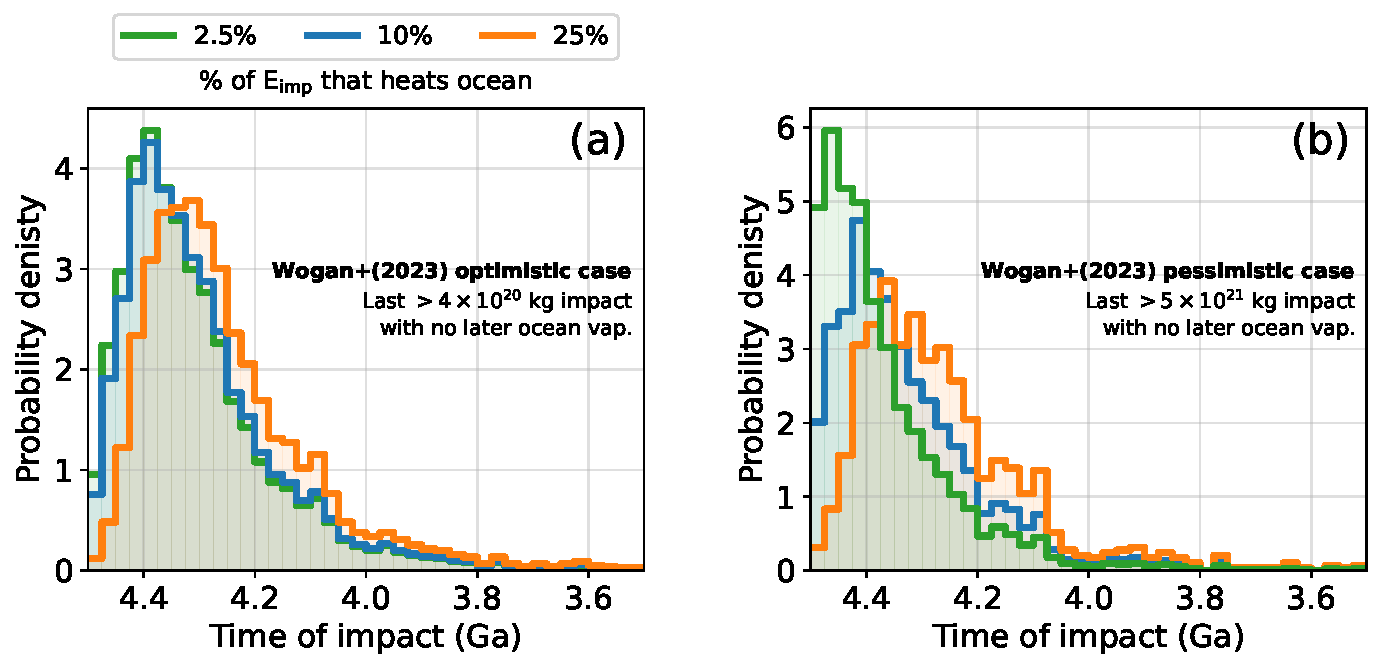
\includegraphics[width=0.85\textwidth]{figures/timing_sensitivity.pdf}
  \caption{Similar to Figure \ref{fig:time_and_mass}, except we consider different values for the fraction of impactor energy that heats the ocean.}
  \label{fig:timing_sensitivity}
\end{figure}

Overall, uncertainty in the impact properties required to vaporize the ocean has a small effect on our qualitative conclusions. Regardless of $f_\mathrm{E,vap}$, the origin of life on Earth from an impact does not appear to be a fluke (Figure \ref{fig:probabilities_of_impacts_sens}) and biopoiesis is preferred early in the Hadean with uncertainty spanning the entire eon (Figure \ref{fig:timing_sensitivity}). However, it is conceivable that a more complete understanding $f_\mathrm{E,vap}$ as a function of impact angle and other impact parameters could change these results.

\bibliography{bib}
\bibliographystyle{aasjournal}

\end{document}
